\documentclass[11pt, oneside, numbers=noenddot]{scrbook}  
\input{./includes/htl_definintions.tex}	

% --------------------------------------------------------
% Allgmeine Informationen über die Arbeit, wie Titel, 
% Autoren, Betreuer, etc. werden hier definiert
% --------------------------------------------------------



% Titel der Arbeit:
\def\htlArbeitsthema{Thema der Diplomarbeit}

% Schuljahr und Schwerpunkt
\def\htlSchuljahr{2025/2026}
\def\htlFachrichtung{Elektronik und technische Informatik}
\def\htlSchwerpunkt{Communications}

% Betreuer
\def\htlBetreuer{Dipl.-Ing. Lukas Lämpel}

% Ort
\def\htlOrt{Braunau/Inn}

% Autoren (Name, Klasse, Initialen)
\def\htlAuthorNameA{Max Mustermann}
\def\htlAuthorClassA{5BHELS}
\def\authorInitialsA{MM}

\def\htlAuthorNameB{Frieda Fröhlich}
\def\htlAuthorClassB{5BHELS}
\def\authorInitialsB{FF}

% Kann bei Bedarf erweitert werden, z.B. für Gruppenarbeiten mit mehr als 2 Personen
% \def\htlAuthorNameC{Fritz Einstein}
% \def\htlAuthorClassC{5BHELS}
% \def\authorInitialsC{FE}

% \def\htlAuthorNameD{Eva Auer}
% \def\htlAuthorClassD{5BHELS}
% \def\authorInitialsD{EA}

% Die Initialen werden verwendet um anzuzeigen wer welches Kapitel
% erstellt hat.

% Die Befehle \authorA - \authorD werden in den Kapitelüberschriften angefügt
\def\authorA{\textmd{\textsuperscript{\authorInitialsA}}}
\def\authorB{\textmd{\textsuperscript{\authorInitialsB}}}
% \def\authorC{\textmd{\textsuperscript{\authorInitialsC}}}
% \def\authorD{\textmd{\textsuperscript{\authorInitialsD}}}	

\begin{document}


% --------------------------------------------------------
% Deckblatt, Eidesstattliche Erklärung, Abstract, etc. 
% --------------------------------------------------------
\pagenumbering{roman}	
		
% !TEX root = ../diplomarbeit.tex

%	########################################################
% 							Deckblatt
%	########################################################


\titlehead{%
\begin{minipage}[c]{0.20\linewidth}

\includegraphics[width=0.8\linewidth]{media/images/htl_c_cmyk_rein}
\end{minipage}
\begin{minipage}[c]{0.5\linewidth}
\begin{center}
{\bfseries\sffamily\large Höhere  technische  Bundeslehranstalt\\
und  Bundesfachschule\\
{\normalsize im Hermann Fuchs Bundesschulzentrum} }
\end{center}
\end{minipage}
\begin{minipage}[c]{0.2\linewidth}
\hfill 
\includegraphics[width=0.8\linewidth]{media/images/htl-bildung-mit-zukunft}
\end{minipage}\\
}
\title{\vspace{4em}\htlArbeitsthema}
\subtitle{ {\Large Diplomarbeit}\\[1em]Fachrichtung, Schulautonomer Schwerpunkt\\ \htlFachrichtung, \htlSchwerpunkt}



\author{\\[3.5em] 
\emph{ausgeführt im Schuljahr \htlSchuljahr\ von:} \\[1em] 
\ifdef{\htlAuthorNameA}{\htlAuthorNameA, \htlAuthorClassA\\[1ex]}{}%
\ifdef{\htlAuthorNameB}{\htlAuthorNameB, \htlAuthorClassB\\[1ex]}{}%
\ifdef{\htlAuthorNameC}{\htlAuthorNameC, \htlAuthorClassC\\[1ex]}{}%
\ifdef{\htlAuthorNameD}{\htlAuthorNameD, \htlAuthorClassD\\[1ex]}{}%
\\[3em]
\emph{Betreuer:} \\[1em]
 \htlBetreuer
}
\date{\vspace{3\baselineskip}\today}

\begin{titlepage}	
\maketitle
\end{titlepage}

% !TEX root = ../diplomarbeit.tex

\chapter*{Eidesstattliche Erklärung}


\ifdef{\htlAuthorNameB}{%
% Mehrere Autoren
Wir erklären an Eides statt, dass wir die vorliegende Diplomarbeit selbstständig und ohne fremde Hilfe verfasst, andere als angegebene Quellen und Hilfsmittel nicht direkt benutzt und die benutzten Quellen wörtlich und inhaltlich entnommenen Stellen als solche erkenntlich gemacht haben.\newline
}{%
% Ein Autor
Ich erkläre an Eides statt, dass ich die vorliegende Diplomarbeit selbstständig und ohne fremde Hilfe verfasst, andere als angegebene Quellen und Hilfsmittel nicht direkt benutzt und die benutzten Quellen wörtlich und inhaltlich entnommenen Stellen als solche erkenntlich gemacht habe.\newline  
}%

\vspace{3cm}

\begin{tabularx}{\textwidth}{l p{1cm} l p{1cm} X}

\ifdef{\htlAuthorNameA}{%
\htlOrt, \todayshort & & \htlAuthorNameA & & \hrulefill \\
\emph{Ort, Datum} & & \emph{Name} & & \emph{Unterschrift} \vspace{2cm}\\ 
}{}

\ifdef{\htlAuthorNameB}{%
\htlOrt, \todayshort & & \htlAuthorNameB & & \hrulefill \\
\emph{Ort, Datum} & & \emph{Name} & & \emph{Unterschrift} \vspace{2cm}\\ 
}{}

\ifdef{\htlAuthorNameC}{%
\htlOrt, \todayshort & & \htlAuthorNameC & & \hrulefill \\
\emph{Ort, Datum} & & \emph{Name} & & \emph{Unterschrift} \vspace{2cm}\\ 
}{}

\ifdef{\htlAuthorNameD}{%
\htlOrt, \todayshort & & \htlAuthorNameD & & \hrulefill \\
\emph{Ort, Datum} & & \emph{Name} & & \emph{Unterschrift} \vspace{2cm}\\ 
}{}

\end{tabularx}



% !TEX root = ../diplomarbeit.tex

\chapter*{Abstract}
\addcontentsline{toc}{chapter}{Abstract}

\emph{Das Abstract ist eine prägnante Zusammenfassung der gesamten Arbeit in englischer Sprache. Es umfasst typischerweise 150--250 Wörter und beschreibt das Problem, die verwendete Methodik, die wichtigsten Ergebnisse und die Schlussfolgerungen. Das Abstract ermöglicht Lesenden eine schnelle Einschätzung der Relevanz der Arbeit.}

% --------------------------------------------------------
\placeholderbox{Example}{%
Modern software development faces significant challenges in managing dependencies across large-scale projects, with version conflicts consuming substantial developer time. Existing dependency management tools provide automatic updates but fail to consider semantic compatibility at the API level, leading to runtime errors and costly hotfixes.

This thesis presents an intelligent dependency analyzer that leverages static code analysis to detect actual API usage patterns and automatically suggest compatible library versions. The system combines abstract syntax tree analysis with a machine learning classifier trained on 50,000 real-world dependency conflicts.

Evaluation on ten open-source projects (10,000--100,000 lines of code) demonstrates that the analyzer identifies 94\,\% of breaking changes before integration, with an average analysis time of 3.2 minutes per project. The false positive rate was reduced to 8\,\% compared to 23\,\% in existing tools.

The proposed solution significantly reduces integration risks and accelerates development cycles. Future work will extend support to dynamic languages and incorporate runtime behavior analysis.
}

\chapter*{Kurzfassung}
\addcontentsline{toc}{chapter}{Kurzfassung}

\emph{Die Kurzfassung ist eine prägnante Zusammenfassung der gesamten Arbeit in deutscher Sprache. Sie umfasst typischerweise 150--250 Wörter und beschreibt das Problem, die verwendete Methodik, die wichtigsten Ergebnisse und die Schlussfolgerungen. Die Kurzfassung ermöglicht Lesenden eine schnelle Einschätzung der Relevanz der Arbeit.}

\placeholderbox{Beispiel}{%
Die moderne Softwareentwicklung steht vor erheblichen Herausforderungen bei der Verwaltung von Abhängigkeiten in großangelegten Projekten, wobei Versionskonflikte erhebliche Entwicklerzeit binden. Bestehende Dependency-Management-Tools bieten zwar automatische Updates, berücksichtigen jedoch nicht die semantische Kompatibilität auf API-Ebene, was zu Laufzeitfehlern und kostspieligen Hotfixes führt.

Diese Diplomarbeit präsentiert einen intelligenten Dependency-Analyzer, der mittels statischer Code-Analyse tatsächliche API-Nutzungsmuster erfasst und automatisch kompatible Bibliotheksversionen vorschlägt. Das System kombiniert Abstract-Syntax-Tree-Analyse mit einem Machine-Learning-Klassifikator, der mit 50.000 realen Abhängigkeitskonflikten trainiert wurde.

Die Evaluierung an zehn Open-Source-Projekten (10.000--100.000 Zeilen Code) zeigt, dass der Analyzer 94\,\% der Breaking Changes vor der Integration identifiziert, bei einer durchschnittlichen Analysezeit von 3,2 Minuten pro Projekt. Die False-Positive-Rate wurde gegenüber bestehenden Tools von 23\,\% auf 8\,\% reduziert.

Die vorgeschlagene Lösung reduziert Integrationsrisiken signifikant und beschleunigt Entwicklungszyklen. Zukünftige Arbeiten werden die Unterstützung dynamischer Sprachen erweitern und Laufzeitverhaltensanalyse integrieren.
}

\tableofcontents

% --------------------------------------------------------
% Beispielhafte Inhalte, wie Zitate, Abbildungen, 
% Quelltext, etc. 
% --------------------------------------------------------
% !TEX root = ../diplomarbeit.tex

% --------------------------------------------------------
%   INFO: Zitieren, Abbildungen, Listing
%	--------------------------------------------------------


%	--------------------------------------------------------
%   Überschrift, Inhaltsverzeichnis
%	--------------------------------------------------------
\chapter*{Beispielhafte Inhalte: Zitieren, Abbildungen, Quelltext}\label{ref:zitieren}
\markboth{Beispielhafte Inhalte: Zitieren, Abbildungen, Quelltext}{Mein Kapitel}
\addcontentsline{toc}{chapter}{Beispielhafte Inhalte: Zitieren, Abbildungen, Quelltext}

\placeholderbox{Hinweis}{
\subsection*{Achtung!}
In diesem Kapitel ist nicht Teil der Diplomarbeit, sondern dient lediglich der Veranschaulichung, wie Abbildungen, Zitate und Quelltext zu verwenden sind.
\newline\newline
Die Zitate, Abbildungen und Listings werden automatisch in das Quellen- und Abbildungsverzeichnis übernommen. 
Das Literatur-, Abbildungs- und Listingsverzeichnis sind am Ende der Arbeit zu finden.
\newline\newline
Auch beschrieben wird, wie mit KI-generierten Inhalten umzugehen ist. Alle KI-generierten Inhalte müssen als solche gekennzeichnet werden, um Transparenz zu gewährleisten.
}

%	--------------------------------------------------------
% 	Inhalt 
%	--------------------------------------------------------

% --------------------------------------------------------
% TODO: Beschreibung für diesen Abschnitt hinzufügen
% --------------------------------------------------------
\section*{Abbildungen}\label{ref:abbildungen}

Abbildung sind mit einer Abbildungsnummer und einer Unterschrift zu versehen die kurz die Abbildung beschreibt. 
Abbildungen gehören zum umgebenden Text und müssen dort erwähnt werden.

\placeholderbox{Beispiel}{
Beispiel: In Abbildung \ref{htl01} wird das Logo der HTL Braunau dargestellt.
}

Wird auf eine Abbildung referenziert die sich weiter von der aktuellen Textstelle entfernt befindet so kann auch die Seitennummer hinzugefügt werden.

\placeholderbox{Beispiel}{
Beispiel: Siehe Abbildung \ref{htl01} auf Seite \pageref{htl01}.
}


%	--------------------------------------------------------
%	Eine Abbildung
\begin{figure}[H]
	\centering
	
\includegraphics[width=0.3\textwidth]{./media/images/htl_c_cmyk_rein.pdf}
  	\caption{Logo der HTL Braunau.}
  	\label{htl01}
\end{figure}


%	--------------------------------------------------------
%	Zwei Abbildungen

\begin{figure}[H]
  \centering
  \subfloat[Logo der HTL Braunau.]{\label{fig:logo_a}
\includegraphics[width=.25\textwidth]{./media/images/htl_c_cmyk_rein.pdf}}
  \qquad
  \subfloat[Logo der HTL Braunau.]{\label{fig:logo_b}
\includegraphics[width=.25\textwidth]{./media/images/htl_c_cmyk_rein.pdf}}
  \label{fig:canvas_01}
  % caption - In eckigen Klammern: Text für das Abbildungsverzeichnis
  \caption[Zwei Logos der HTL Braunau]{Zwei Logos der HTL Braunau in einer Abbildung zusammengefasst.}
\end{figure}


%	--------------------------------------------------------
%	Drei Abbildungen
\begin{figure}[H]
  \centering
  \subfloat[Logo]{\label{fig:logo_c}
\includegraphics[width=.15\textwidth]{./media/images/htl_c_cmyk_rein.pdf}}
  \qquad
  \subfloat[Logo]{\label{fig:logo_d}
\includegraphics[width=.15\textwidth]{./media/images/htl_c_cmyk_rein.pdf}}
\qquad
  \subfloat[Logo]{\label{fig:logo_e}
\includegraphics[width=.15\textwidth]{./media/images/htl_c_cmyk_rein.pdf}}
  \label{fig:canvas_04}
\caption[Drei Logos der HTL Braunau]{Dreimal das Logo der HTL Braunau.}
\end{figure}


% --------------------------------------------------------
%   Zitate, Quellen, Fußnoten
% --------------------------------------------------------
\section*{Zitate, Quellen, Fußnoten}

Zitation dient der Nachvollziehbarkeit und ist verpflichtend, sobald fremde
Gedanken, Daten oder Formulierungen verwendet werden. Verwenden Sie im gesamten
Dokument eine einheitliche Zitierweise (z. B. numerische Zitate in eckigen
Klammern) und verweisen Sie immer auf das Literaturverzeichnis.

\subsection* {Allgemeine Regeln}

\textbf{Kurzregeln:}
\begin{itemize}
  \item Direkte Zitate sind selten und müssen wörtlich übernommen werden.
  \item Paraphrasen sind bevorzugt, aber ebenfalls zu belegen.
  \item Längere Zitate werden als Blockzitat gesetzt.
  \item Verkürzungen in Zitaten werden mit [\ldots] gekennzeichnet.
\end{itemize}

\placeholderbox{Beispiel für Quellenangabe}{
Quellenangaben gehören immer ins Literaturverzeichnis, das automatisch aus den verwendeten Zitationen erstellt wird \cite{bib:wikilitverz}.
}

\placeholderbox{Beispiel für Quellenangabe}{
Das Verwenden fremden Gedankenguts ohne Quellenangabe ist ein Plagiat und kann
rechtliche Folgen haben \cite{bib:wikiplagiat}.
}
\subsection*{Praktische Beispiele}

\placeholderbox{Längeres Zitat mit Verkürzung und anschließender Einordnung}{
\textbf{Navigation in Single-Page-Websites}

\begin{quotation}
\noindent
\emph{\glqq We tend to think of navigating a website as clicking from page-to-page via some kind of global navigation [\ldots] When it comes to a single page, we often think scrolling is the one and only way to move from one end to the next.\grqq}~\cite{bib:bradley}
\end{quotation}

Der Autor betont, dass Nutzer:innen Navigation oft mit klassischen Menüs gleichsetzen. Für unser Projekt bedeutet das, dass bei One-Page-Designs klare Orientierungspunkte (z. B. Abschnittsmarker oder
Kurz-Links) notwendig sind, um den roten Faden der Nutzung zu sichern.
}

\subsection*{Kurzregeln zu Footnotes vs. Zitation:}

\begin{itemize}
  \item Zitate verwenden, wenn eine Aussage, Zahl oder Idee aus einer
  Quelle stammt und nachprüfbar belegt werden muss.
  \item Fußnoten verwenden, wenn eine kurze Nebeninformation, ein Begriffshinweis oder eine ergänzende Erklärung den Lesefluss sonst stören würde.
\end{itemize}

\placeholderbox{Kurze Nebeninformationen als Fußnote}{
Die Implementierung erfolgte in Python 3.11\footnote{Verwendet wurde die offizielle Distribution von python.org, Version 3.11.4}, da diese Version zum Zeitpunkt der Entwicklung die aktuellste stabile Version war.
}

\placeholderbox{Begriffserklärung als Fußnote}{
In diesem Abschnitt wird der Begriff \emph{NPR} verwendet.\footnote{NPR steht für \emph{Non-photorealistic
Rendering} und beschreibt Techniken, die bewusst nicht fotorealistisch wirken.}
}

\placeholderbox{Methodischer Hinweis als Fußnote}{
Die Messwerte wurden in einer Testumgebung erhoben.\footnote{Die Tests liefen auf einem isolierten System ohne
Produktivlast; Ergebnisse sind daher nur bedingt auf den Live-Betrieb
übertragbar.}
}



% --------------------------------------------------------
%   Künstliche Intelligenz in akademischen Arbeiten
% --------------------------------------------------------
\subsection*{Künstliche Intelligenz in akademischen Arbeiten}

Der Einsatz von KI-Tools (wie Large Language Models, Bildgeneratoren oder Code-Assistenten) nimmt in akademischen Arbeiten zu. Diese Tools können bei Recherche, Ideenfindung, Code-Generierung und Texterstellung unterstützen. 
\textbf{Wichtig:} Jeder Abschnitt oder jede Information, die mit Hilfe von KI erstellt oder wesentlich überarbeitet wurde, muss als \textbf{Fußnote} gekennzeichnet werden. Dies garantiert Transparenz und ermöglicht es dem Leser, die Quellenqualität einzuschätzen.

Die Fußnote sollte folgende Informationen enthalten:
\begin{itemize}
  \item Verwendetes Modell/Tool (z.B. \textit{Claude Haiku 4.5}, \textit{ChatGPT-4}, \textit{GitHub Copilot})
  \item Datum der Anfrage
  \item Kurze Beschreibung des Prompts/der Anfrage
  \item Bearbeitung durch den Autor (falls zutreffend)
\end{itemize}

\placeholderbox{Beispiel für Absatz mit KI-Unterstützung}{
KI-Systeme revolutionieren die Art und Weise, wie wir Informationen verarbeiten und Entscheidungen treffen. Durch ihre Fähigkeit zur Mustererkennung und Datenanalyse ermöglichen sie schnellere und präzisere Lösungen in verschiedensten Anwendungsbereichen.\footnote{Dieser Absatz basiert auf einer Anfrage an Claude Haiku 4.5 vom 12.02.2026 mit dem Prompt: \glqq Schreibe einen einleitenden Absatz über die Auswirkungen von KI auf Informationsverarbeitung und Entscheidungsfindung.\grqq ~Das Ergebnis wurde für akademische Zwecke angepasst und auf Korrektheit überprüft.}
}


Diese Integration von KI in wissenschaftliche Arbeiten erfordert aber kritisches Denken und Verantwortung. Der Autor bleibt für alle verwendeten Inhalte verantwortlich, auch wenn diese mit KI-Unterstützung erstellt wurden.


%	--------------------------------------------------------
%	Listings, Code
%	--------------------------------------------------------

% --------------------------------------------------------
% TODO: Beschreibung für diesen Abschnitt hinzufügen
% --------------------------------------------------------
\section*{Listings, Code}

Quelltext ist ein wesentlicher Bestandteil einer Informatik Diplomarbeit.
Listings werden wie Abbildungen nummeriert und mit einer Unterschrift versehen.
Ebenfalls müssen sie im Text referenziert werden.

\subsection*{Beispiele}

Listing \ref{code:helloworld} auf Seite \pageref{code:helloworld} zeigt ein Hallo Welt Programm.

%	--------------------------------------------------------
%	C++
\begin{minipage}{\linewidth}
\lstinputlisting[language=C++,caption={Mein erstes C-Programm.},label=code:helloworld]{./media/code_snippets/bsp_01.cpp}
\end{minipage}


Das PHP Programm \ref{code:phpread} dient zum ermitteln aller Dateien eines Unterverzeichnisses.

\begin{lstlisting}[language=PHP,caption={Alle Dateinamen ausgeben.},label=code:phpread]
<?php
if ($handle = opendir(realpath(__DIR__ . '/../userimages'))) {
    
    while (false !== ($file = readdir($handle))) {
        echo "$file//";
    }

    closedir($handle);
}
?>
\end{lstlisting}

\begin{lstlisting}[language=JavaScript,caption={Mausposition ermitteln.}]
// Calculates the mouse position.
function getMousePos(canvas, evt) {
	var rect = canvas.getBoundingClientRect();
	return {
		x: evt.clientX - rect.left,
		y: evt.clientY - rect.top
	};
}
\end{lstlisting}


%	--------------------------------------------------------
%	CSS
\lstinputlisting[language=CSS,caption={Kurzer CSS--Quelltext.}]{./media/code_snippets/bsp.css}


%	--------------------------------------------------------
%	HTML
\lstinputlisting[language=HTML,caption={HTML--Quelltext}]{./media/code_snippets/bsp.html}


%	--------------------------------------------------------
%	HTML
\lstinputlisting[language=JavaScript,caption={JavaScript--Quelltext}]{./media/code_snippets/bsp.js}







% --------------------------------------------------------
% Einzelnen Kapitel der Arbeit.
% Die Kapitel selbst befinden sich im Ordner "chapters" 
% und können dort bearbeitet werden.
% --------------------------------------------------------
\pagenumbering{arabic}	


% !TEX root = ../diplomarbeit.tex

\chapter{Einleitung\authorA}

In diesem Kapitel werden die Ziele dieser Diplomarbeit festgehalten. Die Gliederung der Arbeit wird durch einen kurzen Überblick über die Kapitel beschrieben.

\section{Motivation, Problemstellung und Zielsetzung}

% Dieser Abschnitt erläutert die Motivation für die Themenwahl, beschreibt das zu lösende Problem und definiert die konkreten Ziele der Arbeit. Eine klare Problemstellung und explizite Zielsetzung sind wesentlich, um den Rahmen der Arbeit abzustecken und die Erfolgskriterien zu definieren.

\placeholderbox{Beispiel}{%
\subsection*{Motivation}
In der modernen Softwareentwicklung stellt die Verwaltung von Abhängigkeiten in großen Projekten eine zunehmende Herausforderung dar. Entwicklerteams verbringen durchschnittlich 20\,\% ihrer Arbeitszeit mit der Analyse und Behebung von Versionskonflikten zwischen Bibliotheken.

\subsection*{Problemstellung}
Bestehende Dependency-Management-Tools bieten zwar automatische Aktualisierungen an, berücksichtigen jedoch nicht die semantische Kompatibilität auf API-Ebene. Dies führt zu Breaking Changes, die erst zur Laufzeit erkennbar werden und kostspielige Hotfixes erfordern.

\subsection*{Zielsetzung}
Ziel dieser Arbeit ist die Entwicklung eines intelligenten Dependency-Analyzers, der mittels statischer Code-Analyse die tatsächliche API-Nutzung erfasst und automatisch kompatible Versionen vorschlägt. Das System soll mindestens 90\,\% der Breaking Changes bereits vor der Integration erkennen und die Analysezeit unter 5 Minuten für typische Projekte halten.
}




\section{Gliederung der Arbeit}

% Dieser Abschnitt gibt einen Überblick über den Aufbau der Arbeit und beschreibt kurz den Inhalt der einzelnen Kapitel. Dies ermöglicht Lesenden eine schnelle Orientierung und zeigt die logische Struktur der Argumentation auf.

\placeholderbox{Beispiel}{%
Die vorliegende Arbeit gliedert sich in sieben Kapitel:\\

\textbf{Kapitel 1 -- Einleitung} führt in die Thematik ein, beschreibt die Problemstellung und definiert die Zielsetzung der Arbeit.

\textbf{Kapitel 2 -- Grundlagen} vermittelt das notwendige theoretische Fundament, definiert zentrale Begriffe und stellt den aktuellen Stand der Technik dar.

\textbf{Kapitel 3 -- Konzepte} präsentiert die entwickelten Lösungsansätze, beschreibt die Systemarchitektur und begründet getroffene Designentscheidungen.

\textbf{Kapitel 4 -- Implementierung} dokumentiert die technische Umsetzung, erläutert kritische Implementierungsdetails und beschreibt verwendete Algorithmen.

\textbf{Kapitel 5 -- Prototyp und Evaluation} stellt den entwickelten Prototyp vor, beschreibt durchgeführte Tests und evaluiert die Ergebnisse hinsichtlich der definierten Zielsetzung.

\textbf{Kapitel 6 -- Zusammenfassung und Ausblick} fasst die wichtigsten Erkenntnisse zusammen, reflektiert kritisch die Ergebnisse und skizziert mögliche Weiterentwicklungen.

\textbf{Kapitel 7 -- Projektmanagement} dokumentiert die Projektorganisation, Aufgabenverteilung und den zeitlichen Ablauf der Diplomarbeit.
}
% !TEX root = ../diplomarbeit.tex

\chapter{Grundlagen\authorB}

\section{Begriffsdefinitionen}
% Hier werden zentrale Begriffe definiert und erläutert, um eine einheitliche
% Begrifflichkeit sicherzustellen.

Lorem ipsum dolor sit amet, consectetur adipiscing elit. Aenean viverra eget sapien in fringilla. Proin ac neque non lectus vehicula laoreet in cursus enim. Donec et erat ut erat commodo viverra vitae sed risus.

\section{State of the art}
% Hier wird der aktuelle Stand der Technik bzw. der Forschung zu den relevanten
% Themen beschrieben.

Lorem ipsum~\cite{bib:hanl2004npr} dolor sit amet, consectetur adipiscing elit. Aenean viverra eget sapien in fringilla. Proin ac neque non lectus vehicula laoreet in cursus enim. Donec et erat ut erat commodo viverra vitae sed risus. Etiam tortor justo, placerat in turpis sit amet, egestas tristique libero. Phasellus metus arcu, viverra at interdum ac, convallis non urna. Sed nunc libero, elementum quis ultricies at, vestibulum in arcu.

\section{Theoretische Grundlagen}
% Hier werden mathematische, physikalische oder informatische Prinzipien
% erläutert, die für das Verständnis der Arbeit wichtig sind.

Lorem ipsum dolor sit amet, consectetur adipiscing elit. Aenean viverra eget sapien in fringilla. Proin ac neque non lectus vehicula laoreet in cursus enim. Donec et erat ut erat commodo viverra vitae sed risus. Etiam tortor justo, placerat in turpis sit amet, egestas tristique libero.

\section{Technologische Grundlagen}
% Falls in der Arbeit spezifische Technologien genutzt werden (z. B.
% Programmiersprachen, Hardware, Protokolle), sollten sie hier beschrieben werden.

Lorem ipsum dolor sit amet, consectetur adipiscing elit. Aenean viverra eget sapien in fringilla. Proin ac neque non lectus vehicula laoreet in cursus enim. Donec et erat ut erat commodo viverra vitae sed risus.

\section{Voraussetzungen und Einschränkungen}
% Hier werden die Rahmenbedingungen für die Arbeit definiert.

Lorem ipsum dolor sit amet, consectetur adipiscing elit. Aenean viverra eget sapien in fringilla. Proin ac neque non lectus vehicula laoreet in cursus enim. Donec et erat ut erat commodo viverra vitae sed risus.

% !TEX root = ../diplomarbeit.tex

\chapter{Konzepte\authorA}

% In diesem Kapitel werden verschiedene Lösungsansätze vorgestellt und bewertet.
% Dieses Kapitel ist mit das wichtigste dieser Arbeit.

\section{Konzept A}

Lorem ipsum dolor sit amet, consectetur adipiscing elit. Aenean viverra eget sapien in fringilla. Proin ac neque non lectus vehicula laoreet in cursus enim. Donec et erat ut erat commodo viverra vitae sed risus. Etiam tortor justo, placerat in turpis sit amet, egestas tristique libero.

\section{Konzept B}

Lorem ipsum dolor sit amet, consectetur adipiscing elit. Aenean viverra eget sapien in fringilla. Proin ac neque non lectus vehicula laoreet in cursus enim. Donec et erat ut erat commodo viverra vitae sed risus.

\section{Bewertung und Auswahl}

Lorem ipsum dolor sit amet, consectetur adipiscing elit. Aenean viverra eget sapien in fringilla. Proin ac neque non lectus vehicula laoreet in cursus enim.

% !TEX root = ../diplomarbeit.tex

\chapter{Implementierung}

% Hier wird beschrieben, wie das entwickelte System umgesetzt wurde, welche
% Technologien verwendet wurden und welche Herausforderungen auftraten.

Dieses Kapitel dokumentiert die praktische Umsetzung der im Konzeptteil beschriebenen Lösung. Es werden die gewählte Architektur, zentrale Komponenten, verwendete Technologien sowie besondere Implementierungsentscheidungen und Herausforderungen nachvollziehbar dargestellt.


% !TEX root = ../diplomarbeit.tex

\section{\emph{Beispiel:} Hardware\authorA}

% Hier beschreibt Autor A seinen Teil der Implementierung.
% Welche Technologien verwendet wurden und welche Herausforderungen auftraten.

\subsection{Implementierungsdetails}

\emph{Hier werden die konkrete technische Umsetzung der Systemkomponenten sowie wichtige Designentscheidungen beschrieben. Code-Snippets, UML-Diagramme und Erklärungen zu kritischen Algorithmen verdeutlichen die Implementierung.}

\placeholderbox{Beispiel}{%
Die Kernkomponente analysiert Eingabedaten durch einen dreistufigen Prozess: (1) Daten-Validierung mit JSON-Schema, (2) Transformation mittels einer Custom-Pipeline mit Pluggable-Architektur, (3) Ausgabe-Serialisierung in mehreren Formaten. Die Daten-Validierung wurde als Middleware implementiert, um Fehler früh zu erkennen. Besondere Aufmerksamkeit galt der Fehlerbehandlung mit aussagekräftigen Fehlermeldungen für End-User sowie detaillierten Logs für Developer.%
    %
    \newline\newline
    ...
}

\subsection{Verwendete Technologien}

\emph{Dieser Abschnitt listet alle eingesetzten Programmiersprachen, Frameworks, Bibliotheken und Tools auf und begründet deren Auswahl. Die Darstellung erfolgt strukturiert mit konkreten Versionsangaben und Einsatzzwecken.}

\placeholderbox{Beispiel}{%
\textbf{Backend:} Node.js 18.14.0 mit Express.js 4.18.2 für schnelle API-Entwicklung; Mongoose 7.0.0 für die MongoDB-Integration. Die Wahl fiel auf Node.js wegen der Performance und dem großen Ökosystem.

\textbf{Frontend:} React 18.2.0 mit TypeScript 4.9 für Type-Safety; Material-UI 5.11 für konsistentes Design. React wurde gewählt für Component-Reusability und Virtual DOM Performance.%
    %
    \newline\newline
    ...
}


\section{\emph{Beispiel:} Frontend\authorA}

\subsection{Implementierungsdetails}

\ldots

\subsection{Verwendete Technologien}

\ldots


% !TEX root = ../diplomarbeit.tex

\section{\emph{Beispiel:} Backend und Datenhaltung\authorB}

% Hier beschreibt Autor B seinen Teil der Implementierung.
% Welche Technologien verwendet wurden und welche Herausforderungen auftraten.

\subsection{Implementierungsdetails}

\ldots

\subsection{Verwendete Technologien}

\ldots

% !TEX root = ../diplomarbeit.tex

\chapter{Prototyp und Ergebnisse\authorA}

Dieses Kapitel stellt den entwickelten Prototyp vor und beschreibt die durchgeführten Tests sowie die erzielten Ergebnisse. Ziel ist es, die Funktionsfähigkeit der Lösung anhand konkreter Szenarien zu demonstrieren und die Resultate in Bezug auf die Zielsetzung zu bewerten.


% !TEX root = ../diplomarbeit.tex

\section{\emph{Beispiel:} Hardware\authorA}

% Hier beschreibt Autor A seinen Teil des Prototyps.
% Beschreibung der Umsetzung und durchgeführten Tests.

% --------------------------------------------------------
% Entwicklung und Funktionalitäten des Prototyps
% --------------------------------------------------------
\subsection{Beschreibung des Prototyps}

\emph{Hier wird der entwickelte Prototyp mit seinen Funktionen, der Benutzeroberfläche und den umgesetzten Kernfunktionalitäten vorgestellt. Screenshots, Ablaufdiagramme und Beschreibungen der Benutzerinteraktion dokumentieren den aktuellen Entwicklungsstand.}

\placeholderbox{Beispiel}{%
Der Prototyp wurde als Web-Anwendung mit React (Frontend) und Node.js (Backend) implementiert. Die Benutzeroberfläche besteht aus drei Hauptkomponenten: (1) ein Eingabebereich für Konfigurationsparameter, (2) eine Visualisierungskomponente für Echtzeitdaten und (3) ein Export-Panel für Ergebnisse. Die Anwendung arbeitet vollständig offline und speichert Daten lokal in IndexedDB. Die Kernfunktionalitäten wurden durch 42 Unit-Tests validiert.%
    %
    \newline\newline
    ...
}

% --------------------------------------------------------
% Gewählte Testverfähren und Ergebnisse
% --------------------------------------------------------
\subsection{Tests und Evaluierung}

\emph{Dieser Abschnitt beschreibt die durchgeführten Tests (Unit-Tests, Integrationstests, Benutzertests) sowie deren Ergebnisse. Die Evaluierung bewertet, ob die definierten Anforderungen erfüllt wurden und identifiziert Verbesserungspotenziale.}

\placeholderbox{Beispiel}{%
Folgende Testabdeckung wurde durchgeführt: (1) Unit-Tests für alle kritischen Funktionen mit 98,1\,\% Erfolgsquote, (2) Integrationstests mit realen Eingabedaten zeigten eine durchschnittliche Verarbeitungszeit von 2,3 Sekunden, (3) Usability-Tests mit 8 Testnutzern erreichten einen SUS-Wert von 72 Punkten. Browser-Kompatibilität wurde auf Chrome, Firefox und Safari getestet. Ein kritischer Bug in der Datenvalidierung wurde identifiziert und behoben.%
    %
    \newline\newline
    ...
}

% --------------------------------------------------------
% Erreichte Ergebnisse und Metriken
% --------------------------------------------------------
\subsection{Ergebnisse}

\emph{Dieser Abschnitt fasst die wichtigsten Ergebnisse der Evaluierung zusammen. Die Resultate werden anhand quantitativer Metriken sowie qualitativer Beobachtungen dargestellt und in Bezug zu den in der Zielsetzung definierten Anforderungen bewertet.}

\placeholderbox{Beispiel}{
    Bei der Durchführung von insgesamt 42 Unit-Tests erreichte der Prototyp eine Erfolgsquote von 98,1\,\%. Die durchschnittliche Antwortzeit bei typischen Anwendungsfällen betrug 2,3 Sekunden, was die Anforderung von unter 5 Sekunden deutlich erfüllt. %
    %
    \newline\newline
    ...
}


\section{\emph{Beispiel:} Frontend\authorA}

\subsection{Beschreibung des Prototyps}

\ldots

\subsection{Tests und Evaluierung}

\ldots

\subsection{Ergebnisse}

\ldots

% !TEX root = ../diplomarbeit.tex

\section{\emph{Beispiel:} Backend und Datenhaltung\authorB}

% Hier beschreibt Autor B seinen Teil des Prototyps.
% Beschreibung der Umsetzung und durchgeführten Tests.

\subsection{Beschreibung des Prototyps}

\ldots

\subsection{Tests und Evaluierung}

\ldots

\subsection{Ergebnisse}

\ldots
% !TEX root = ../diplomarbeit.tex

\chapter{Conclusion\authorA}

% Hier werden die Ergebnisse zusammengefasst und ein Fazit gezogen. Außerdem
% können zukünftige Entwicklungen oder offene Fragen angesprochen werden.

\section{Zusammenfassung}

Lorem ipsum dolor sit amet, consectetur adipiscing elit. Aenean viverra eget sapien in fringilla. Proin ac neque non lectus vehicula laoreet in cursus enim. Donec et erat ut erat commodo viverra vitae sed risus. Etiam tortor justo, placerat in turpis sit amet, egestas tristique libero.

\section{Fazit}

Lorem ipsum dolor sit amet, consectetur adipiscing elit. Aenean viverra eget sapien in fringilla. Proin ac neque non lectus vehicula laoreet in cursus enim.

\section{Ausblick}

Lorem ipsum dolor sit amet, consectetur adipiscing elit. Aenean viverra eget sapien in fringilla. Proin ac neque non lectus vehicula laoreet in cursus enim. Donec et erat ut erat commodo viverra vitae sed risus.

% !TEX root = ../diplomarbeit.tex

\chapter{Projektmanagement}

% --------------------------------------------------------
% Projektplanung und Meilensteine
% --------------------------------------------------------
\section{Planung}

\emph{Dieser Abschnitt dokumentiert die Planung der Diplomarbeit, einschließlich der definierten Meilensteine, Zeitlinie und Aufgabenzuordnung. Der Meilensteinplan zeigt die wichtigsten Zwischenziele und deren geplante Fertigstellung.}

% --------------------------------------------------------
% Terminplanung und Meilensteine
% --------------------------------------------------------
\subsection*{Meilensteinplan}

\placeholderbox{Beispiel}{%
\begin{table}[H]
\centering
\begin{tabularx}{\linewidth}{lXl}
\hline
\textbf{Meilenstein} & \textbf{Beschreibung} & \textbf{Termin} \\
\hline
Requirement-Analyse & Anforderungen definieren und dokumentieren & KW 5 \\
Konzeptphase & Verschiedene Lösungsansätze entwickeln und bewerten & KW 7 \\
Implementierung Phase 1 & Kernfunktionalitäten umsetzen & KW 12 \\
Implementierung Phase 2 & Optimierung und erweiterte Features & KW 14 \\
Prototyp \& Testing & Tests durchführen und Ergebnisse dokumentieren & KW 16 \\
Dokumentation & Diplomarbeit finalisieren & KW 17 \\
Abgabe & Finale Abgabe & KW 18 \\
\hline
\end{tabularx}
\caption{Meilensteinplan der Diplomarbeit}
\label{tab:meilensteinplan}
\end{table}
}

% --------------------------------------------------------
% Bewertung der Zielerreichung
% --------------------------------------------------------
\section{Evaluierung}

\emph{Die Evaluierung dokumentiert, wie die gesetzten Ziele erreicht wurden und welche Anpassungen während der Projektlaufzeit vorgenommen wurden. Sie bietet eine Reflexion über die Projektabwicklung und zeigt eventuelle Abweichungen vom ursprünglichen Plan.}

% --------------------------------------------------------
% Arbeitszeiten und Stundenerfassung Autor A
% --------------------------------------------------------
\section{Zeiterfassung \htlAuthorNameA}

\emph{Die Zeiterfassung dokumentiert die investierte Arbeitszeit pro Projektphase und Woche. Dies ermöglicht eine Nachverfolgung der Ressourcennutzung und dient als Grundlage für zukünftige Zeitschätzungen.}

\placeholderbox{Beispiel}{%
\begin{table}[H]
\centering
\renewcommand{\arraystretch}{1.2}
\begin{tabularx}{\textwidth}{l r r X}
\textbf{KW} & \multicolumn{2}{c}{\textbf{Arbeitszeit [h]}} & \textbf{Aufgabenbeschreibung} \\
 & Schule & Freizeit & \\
\hline
KW22 & 10 & 2 &Anforderungsanalyse, Meetings mit Betreuung \\
KW23 & 10 & 4 & Recherche State of the Art, Literature Review \\
\ldots & \ldots & \ldots & \ldots \\
\hline
\textbf{Summe} & \textbf{204} & \textbf{185} &  \\
\hline
\hline
\end{tabularx}
\caption{Wöchentliche Zeiterfassung \htlAuthorNameB}
\label{tab:zeiterfassung_a}
\end{table}
}

% --------------------------------------------------------
% Unterscrift A
% --------------------------------------------------------
\begin{tabularx}{\textwidth}{l p{1cm} l p{1cm} X}

\htlOrt, \todayshort & & \htlAuthorNameA & & \hrulefill \\
\emph{Ort, Datum} & & & & \emph{Unterschrift} \vspace{2cm}\\ 

\end{tabularx}


% --------------------------------------------------------
% Arbeitszeiten und Stundenerfassung Autor B
% --------------------------------------------------------
\section{Zeiterfassung \htlAuthorNameB}


\emph{Die Zeiterfassung dokumentiert die investierte Arbeitszeit pro Projektphase und Woche. Dies ermöglicht eine Nachverfolgung der Ressourcennutzung und dient als Grundlage für zukünftige Zeitschätzungen.}

\placeholderbox{Beispiel}{%
\begin{table}[H]
\centering
\renewcommand{\arraystretch}{1.2}
\begin{tabularx}{\textwidth}{l r r X}
\textbf{KW} & \multicolumn{2}{c}{\textbf{Arbeitszeit [h]}} & \textbf{Aufgabenbeschreibung} \\
 & Schule & Freizeit & \\
\hline
KW22 & 10 & 2 &Anforderungsanalyse, Meetings mit Betreuung \\
KW23 & 10 & 4 & Recherche State of the Art, Literature Review \\
\ldots & \ldots & \ldots & \ldots \\
\hline
\textbf{Summe} & \textbf{204} & \textbf{185} &  \\
\hline
\hline
\end{tabularx}
\caption{Wöchentliche Zeiterfassung \htlAuthorNameB}
\label{tab:zeiterfassung_b}
\end{table}
}


% --------------------------------------------------------
% Unterscrift B
% --------------------------------------------------------

\begin{tabularx}{\textwidth}{l p{1cm} l p{1cm} X}

\htlOrt, \todayshort & & \htlAuthorNameB & & \hrulefill \\
\emph{Ort, Datum} & & & & \emph{Unterschrift} \vspace{2cm}\\ 

\end{tabularx}


% --------------------------------------------------------
% Anhang, Danksagungen, Literaturverzeichnis, PM, etc.
% --------------------------------------------------------
\appendix

% !TEX root = ../diplomarbeit.tex

\chapter*{Danksagungen}
\addcontentsline{toc}{chapter}{Danksagungen}

\emph{In diesem Kapitel werden alle Personen und Organisationen aufgelistet und bedankt, die zur Entstehung dieser Diplomarbeit beigetragen haben. Dies umfasst fachliche Betreuung, technische Unterstützung, Bereitstellung von Ressourcen und persönliche Unterstützung. Ein aufrichtiger Dank würdigt die Beiträge aller Beteiligten.}

\placeholderbox{Beispiel}{%
An dieser Stelle möchten wir uns herzlich bei allen bedanken, die zum Erfolg dieser Diplomarbeit beigetragen haben:

Unser besonderer Dank gilt unserem Diplomarbeit-Betreuer \htlBetreuer$~$ für seine fachliche Anleitung, seine Geduld und wertvollen Hinweise während des gesamten Projektes. Ebenfalls danken wir dem Team der HTL Braunau für die Bereitstellung der notwendigen Infrastruktur und Ressourcen sowie für die Schaffung eines inspirierenden Lernumfeldes.

Wir danken auch der Firma XYZ für die freundliche Unterstützung bei technischen Fragen und der Bereitstellung von Evaluierungs-Datensätzen. Einen besonderen Dank auch unsere Testnutzer, die ihre Zeit für Usability-Tests gewidmet haben und wertvolles Feedback gegeben haben.

Nicht zuletzt möchten wir unseren Familien und Freunden danken, die uns während des Projektes moralisch unterstützt und Verständnis für unseren Zeiteinsatz aufgebracht haben.
}

\addcontentsline{toc}{chapter}{Listings}
\lstlistoflistings

\addcontentsline{toc}{chapter}{List of Figures}
\listoffigures


\addcontentsline{toc}{chapter}{Bibliography}
\bibliographystyle{plain}
\bibliography{literature}

% !TEX root = ../diplomarbeit.tex

\chapter*{CV} \markboth{CV}{CV}
\addcontentsline{toc}{chapter}{CV}


% --------------------------------------------------------
% Authoreninformationen und Lebenslauf Author A
% --------------------------------------------------------
\htlParagraph{\htlAuthorNameA}

\renewcommand{\arraystretch}{1.2}
\begin{tabularx}{1\textwidth}{@{} l X l @{}}

\emph{Geburtstag, Geburtsort:} & 01.01.1970, Braunau am Inn & 
\multirow{5}{2.5cm}{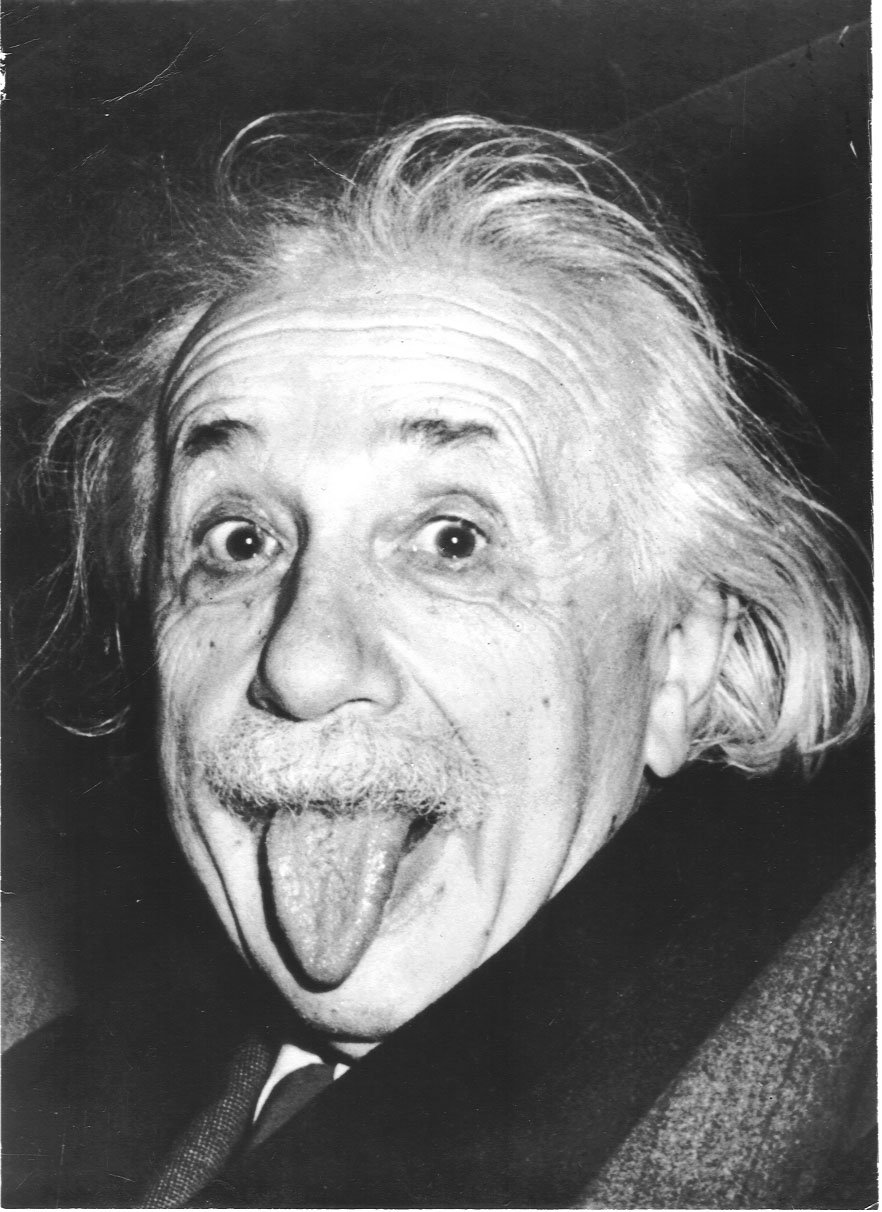
\includegraphics[width=2.5cm]{./media/images/einstein.jpg}
} 
\\
\emph{Schulbildung:} & Volksschule \newline Hauptschule \newline HTL & \\
\emph{Praktika:} & Firmenname, Zeit, Tätigkeit & \\
\emph{Anschrift:} & Strasse Nummer\newline PLZ, Ort\newline Österreich & \\
\emph{E-Mail:} & max@mustermann.com & \\

\end{tabularx}
\\\\

% --------------------------------------------------------
% Authoreninformationen und Lebenslauf Author B
% --------------------------------------------------------
\ifdef{\htlAuthorNameB}{
\htlParagraph{\htlAuthorNameB}

\begin{tabularx}{1\textwidth}{@{} l X l @{}}
\emph{Geburtstag, Geburtsort:} & 01.01.1970, Braunau am Inn & 
\multirow{5}{2.5cm}{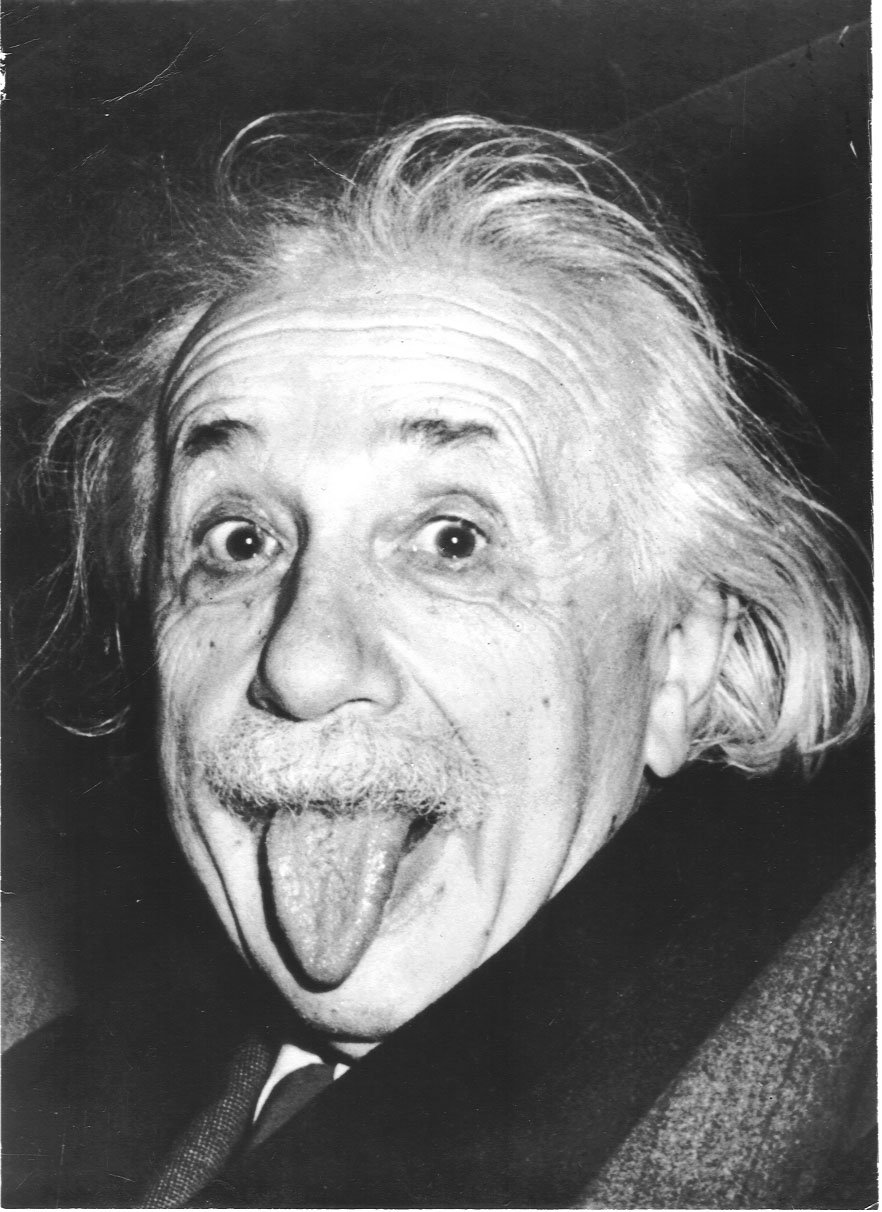
\includegraphics[width=2.5cm]{./media/images/einstein.jpg}
} 
\\
\emph{Schulbildung:} & Volksschule \newline Hauptschule \newline HTL & \\
\emph{Praktika:} & Firmenname, Zeit, Tätigkeit & \\
\emph{Anschrift:} & Strasse Nummer\newline PLZ, Ort\newline Österreich & \\
\emph{E-Mail:} & frieda@froehlich.com & \\

\end{tabularx}
}{}%


% --------------------------------------------------------
% Authoreninformationen und Lebenslauf Author C
% --------------------------------------------------------
\ifdef{\htlAuthorNameC}{
\pagebreak
\htlParagraph{\htlAuthorNameC}

\begin{tabularx}{1\textwidth}{@{} l X l @{}}
\emph{Geburtstag, Geburtsort:} & 01.01.1970, Braunau am Inn & 
\multirow{5}{2.5cm}{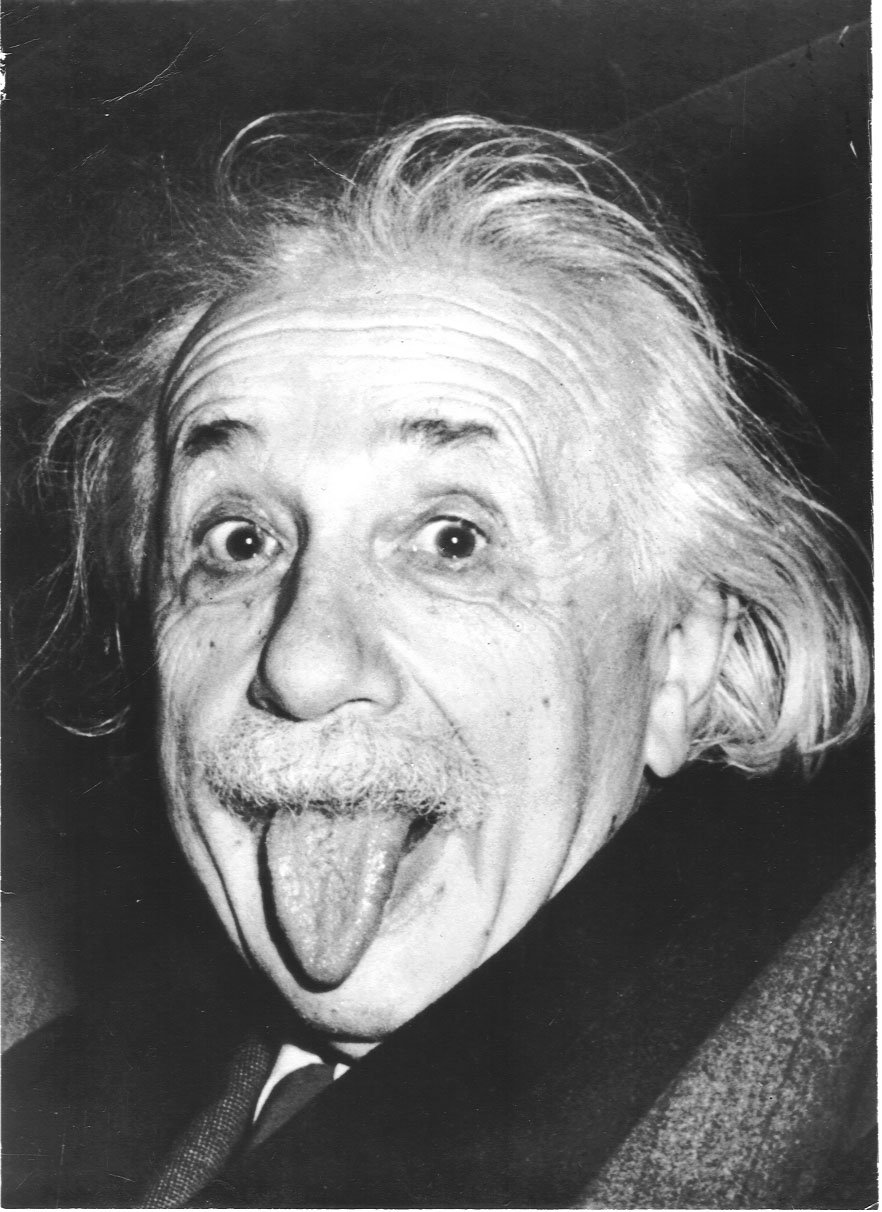
\includegraphics[width=2.5cm]{./media/images/einstein.jpg}
} 
\\
\emph{Schulbildung:} & Volksschule \newline Hauptschule \newline HTL & \\
\emph{Praktika:} & Firmenname, Zeit, Tätigkeit & \\
\emph{Anschrift:} & Strasse Nummer\newline PLZ, Ort\newline Österreich & \\
\emph{E-Mail:} & fritz@einstein.com & \\

\end{tabularx}
\\\\
}{}%


% --------------------------------------------------------
% Authoreninformationen und Lebenslauf Author D
% --------------------------------------------------------
\ifdef{\htlAuthorNameD}{
\htlParagraph{\htlAuthorNameD}

\begin{tabularx}{1\textwidth}{@{} l X l @{}}
\emph{Geburtstag, Geburtsort:} & 01.01.1970, Braunau am Inn & 
\multirow{5}{2.5cm}{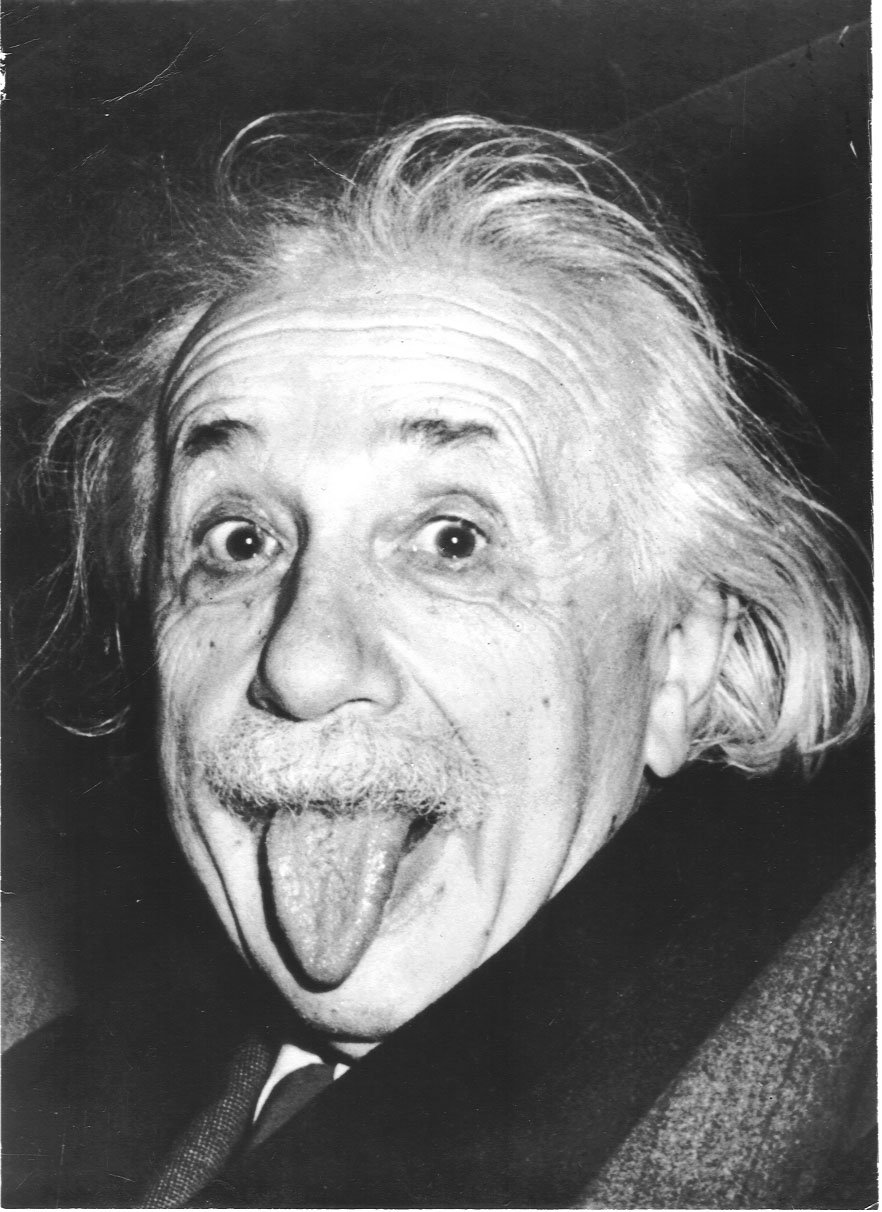
\includegraphics[width=2.5cm]{./media/images/einstein.jpg}
} 
\\
\emph{Schulbildung:} & Volksschule \newline Hauptschule \newline HTL & \\
\emph{Praktika:} & Firmenname, Zeit, Tätigkeit & \\
\emph{Anschrift:} & Strasse Nummer\newline PLZ, Ort\newline Österreich & \\
\emph{E-Mail:} & eva@auer.com & \\

\end{tabularx}
\\\\
}{}%


\end{document}